%SOP Template
% Version 02 Added revision date
% Version 03 Added TOC and acknowledgements
%           New SOP3_alpha.cls
% Version 04 Fix ambiguities about committing

\documentclass[12pt]{../SOP4_alpha}\usepackage[]{graphicx}\usepackage[]{color}
% maxwidth is the original width if it is less than linewidth
% otherwise use linewidth (to make sure the graphics do not exceed the margin)
\makeatletter
\def\maxwidth{ %
  \ifdim\Gin@nat@width>\linewidth
    \linewidth
  \else
    \Gin@nat@width
  \fi
}
\makeatother

\definecolor{fgcolor}{rgb}{0.345, 0.345, 0.345}
\newcommand{\hlnum}[1]{\textcolor[rgb]{0.686,0.059,0.569}{#1}}%
\newcommand{\hlstr}[1]{\textcolor[rgb]{0.192,0.494,0.8}{#1}}%
\newcommand{\hlcom}[1]{\textcolor[rgb]{0.678,0.584,0.686}{\textit{#1}}}%
\newcommand{\hlopt}[1]{\textcolor[rgb]{0,0,0}{#1}}%
\newcommand{\hlstd}[1]{\textcolor[rgb]{0.345,0.345,0.345}{#1}}%
\newcommand{\hlkwa}[1]{\textcolor[rgb]{0.161,0.373,0.58}{\textbf{#1}}}%
\newcommand{\hlkwb}[1]{\textcolor[rgb]{0.69,0.353,0.396}{#1}}%
\newcommand{\hlkwc}[1]{\textcolor[rgb]{0.333,0.667,0.333}{#1}}%
\newcommand{\hlkwd}[1]{\textcolor[rgb]{0.737,0.353,0.396}{\textbf{#1}}}%
\let\hlipl\hlkwb

\usepackage{framed}
\makeatletter
\newenvironment{kframe}{%
 \def\at@end@of@kframe{}%
 \ifinner\ifhmode%
  \def\at@end@of@kframe{\end{minipage}}%
  \begin{minipage}{\columnwidth}%
 \fi\fi%
 \def\FrameCommand##1{\hskip\@totalleftmargin \hskip-\fboxsep
 \colorbox{shadecolor}{##1}\hskip-\fboxsep
     % There is no \\@totalrightmargin, so:
     \hskip-\linewidth \hskip-\@totalleftmargin \hskip\columnwidth}%
 \MakeFramed {\advance\hsize-\width
   \@totalleftmargin\z@ \linewidth\hsize
   \@setminipage}}%
 {\par\unskip\endMakeFramed%
 \at@end@of@kframe}
\makeatother

\definecolor{shadecolor}{rgb}{.97, .97, .97}
\definecolor{messagecolor}{rgb}{0, 0, 0}
\definecolor{warningcolor}{rgb}{1, 0, 1}
\definecolor{errorcolor}{rgb}{1, 0, 0}
\newenvironment{knitrout}{}{} % an empty environment to be redefined in TeX

\usepackage{alltt}
\usepackage{float}
\usepackage{amssymb}
\author{Marc Los Huertos \& Isaac Medina}
\title{Rstudio Projects and Github}
\date{1/16/2018}
\approved{Marc Los Huertos}
\ReviseDate{\today}
\SOPno{10 v.04}

\usepackage{graphicx}
\IfFileExists{upquote.sty}{\usepackage{upquote}}{}
\begin{document}

\maketitle

\section{Scope and Application}

\NP R, RStudio, and Github combine as a resource for data analysis and display.

\NP We explain how these resources can be set up to create collaborative projects using Github repositories. 

\NP We do not expect you to be an expert on how to use R or Rstudio. However, some experience with a computer language will be helpful. 

\section{Summary of Method}

\NP This SOP provides instructions to create Rstudio projects and obtain Github repositories into Rstudio. 

\NP The SOP also provides some guidance on how to troubleshoot should push/pull problems arise.

\NP The use of Github is not always intuitive and we can not cover all of the topics in this SOP. So, you should plan to rely on a wide range on-line resources to help.

\tableofcontents

\newpage

\section{Acknowledgements}

As usual we acknowledge the students who have tried to follow and made suggestions on how to improve this guide. If you have suggestions or edits to improve the document, please let the author(s) know so they can make changes and you can be acknowledged.

The following have made substantial contributions:

\begin{itemize}
\item Aparna Chintapalli
\end{itemize}

\section{Definitions}

\NP RStudio is the user interface for R. Although R by itself is an amazing example of crowd sourcing, where a wide range of staticians and programmers have created a free programming environments with a robust range of statistical packages, the RStudio interface provides a user with the tools to track and publish their analysis process in an effecient and transparent way. 

\NP Local Install versus Server --- R and RStudio can be installed on a local computer/laptop from the CRAN download mirror sites. However, we also have access to the R and RStudio Server installed on the Pomona College mainframe, where you can access it via a web browser. Wow, this is convenient!

\NP GitHub is a web-based Git repository hosting service. 

\NP Version Control is a method to track changes in software, and often in the context of collaborative projects. The final component of R and RStudio is its capacity to create projects (RStudio's terminology) and repositories (Github's terminalogy) that can be shared among collaborators. In particular, the collaboration allows for contributions to be tracked via version control tools. There are a number of ways that we can access these tools, but we'll try to limit the methods to keep the process relatively ``simple''.


\section{Background}

\NP R is a powerful, open source program but combined with RStudio and Github the program becomes an archetype of a program that enables 1) collaboration, 2) transparency, 3 reproducibility, and 3) accessibility: 

\begin{description}
    \item[Collaboration] You can easily collaborate with others and track who contributed to various parts of the repository. When you are working in a team and updating various text and code, it's important to have version control to ensure that you can trace how the text and code was change. 
    
  \item[Transparency] The program allows others to see how you analyzed the data and thus, allows clear access to what you have done.
    
  \item[Reproducibility]  that when you conduct an analysis you can reproduce the results that can be used to validate your results. 
  
  \item[Accessibility] Accessible from any computer via webserver. Becuase we can rely on consistant behavoir and even web-based servers, the operating systems and computer hardware rarely limit what you can do in R.

\end{description}

\NP However, becoming experienced in using these programs is like learning how to walk. We need to approach this process in discrete steps. Some people will experience weeks of mistakes before they are confident in their abilities to use these programs, others will quickly learn to run with the programs. How quickly you can feel comfortable with these programs will depend on many factors, but will be greatly improved by the time you invest!

\NP I recommend reading the following sites to better understand Git and Github

\begin{itemize}
  \item \href{https://www.youtube.com/watch?v=uHYcDQDbMY8}{Rstudio Youtube}
  \item \href{https://www.youtube.com/watch?v=0fKg7e37bQE}{Github Youtube}
  \item \href{http://product.hubspot.com/blog/git-and-github-tutorial-for-beginners}{Github for Beginners}
  \item \href{http://scottchacon.com/2011/08/31/github-flow.html}{Github Fw}
  \item \href{https://guides.github.com/introduction/flow/}{Understanding the GitHub Flow}
  \item \href{http://blog.osteele.com/posts/2008/05/my-git-workflow/}{http://blog.osteele.com/posts/2008/05/my-git-workflow/}
  
\end{itemize}


\section{Interferences}

\NP R has an updated version about every six months. When performing advanced analyses, there are times that new versions will no longer run a code. Thus, older versions of R must be maintained. This is a unheard of issue for new users -- thankfully. It almost never occurs because new users rarely are running advanced codes!

\NP RStudio Server needs a functional network connection. If the network is down, then Rstudio Server is inaccessible. This can be a source of frustration. 

\section{Health and Safety}

\NP Some risks include carpal tunnel syndrome.

\NP Frustation!  After running into errors that seem to baffle you, go for a run, get dinner, or take a nap. Often you'll find a work around after you take a break. 


\subsection*{Safety and Personnnel Protective Equipment}

\NP Good posture and well designed work station

\section{Personnel \& Training Responsibilities}

\NP Researchers using this SOP should be well versed in webbrowser and file storage practices. 

%\NP Researchers using this SOP should be trained for the following SOPs:

\section{Required Materials and Apparati}

\NP Laptop or destop computer

\NP Access to Pomona College's SSO (single sign on) and server

\NP Github account

\NP Patience

%\section{Reagents and Standards}

\section{Estimated Time}

\NP This set up procedure requires 45 minutes.

%\section{Maintaining XX Data}

\section{Introducing Rstudio}

\subsection{RStudio Server Login}

\NP The Rstudio Server is hosted by Pomona College, thus you'll need a Pomona College login. 

\NP For non-Pomona College students, you'll need a new login each semester, which can be obtained from the help desk at Cowart Information Technology Services building.

\NP Depending on your location, you can login to the server with \url{rstudio.campus.pomona.edu} if you are on the Pomona's network (or can use the VPN while off campus). However, if you are off campus and can't use the Pomona network, use this address: \url{rstudio.pomona.edu} from off campus including non-Pomona networks.

\NP From non-Pomona college networks you might get an error (Figure~\ref{fig:privacyerror}). If you get this error, go to Advanced and accept the privacy settings to continue.

\begin{figure}[t]
\centering
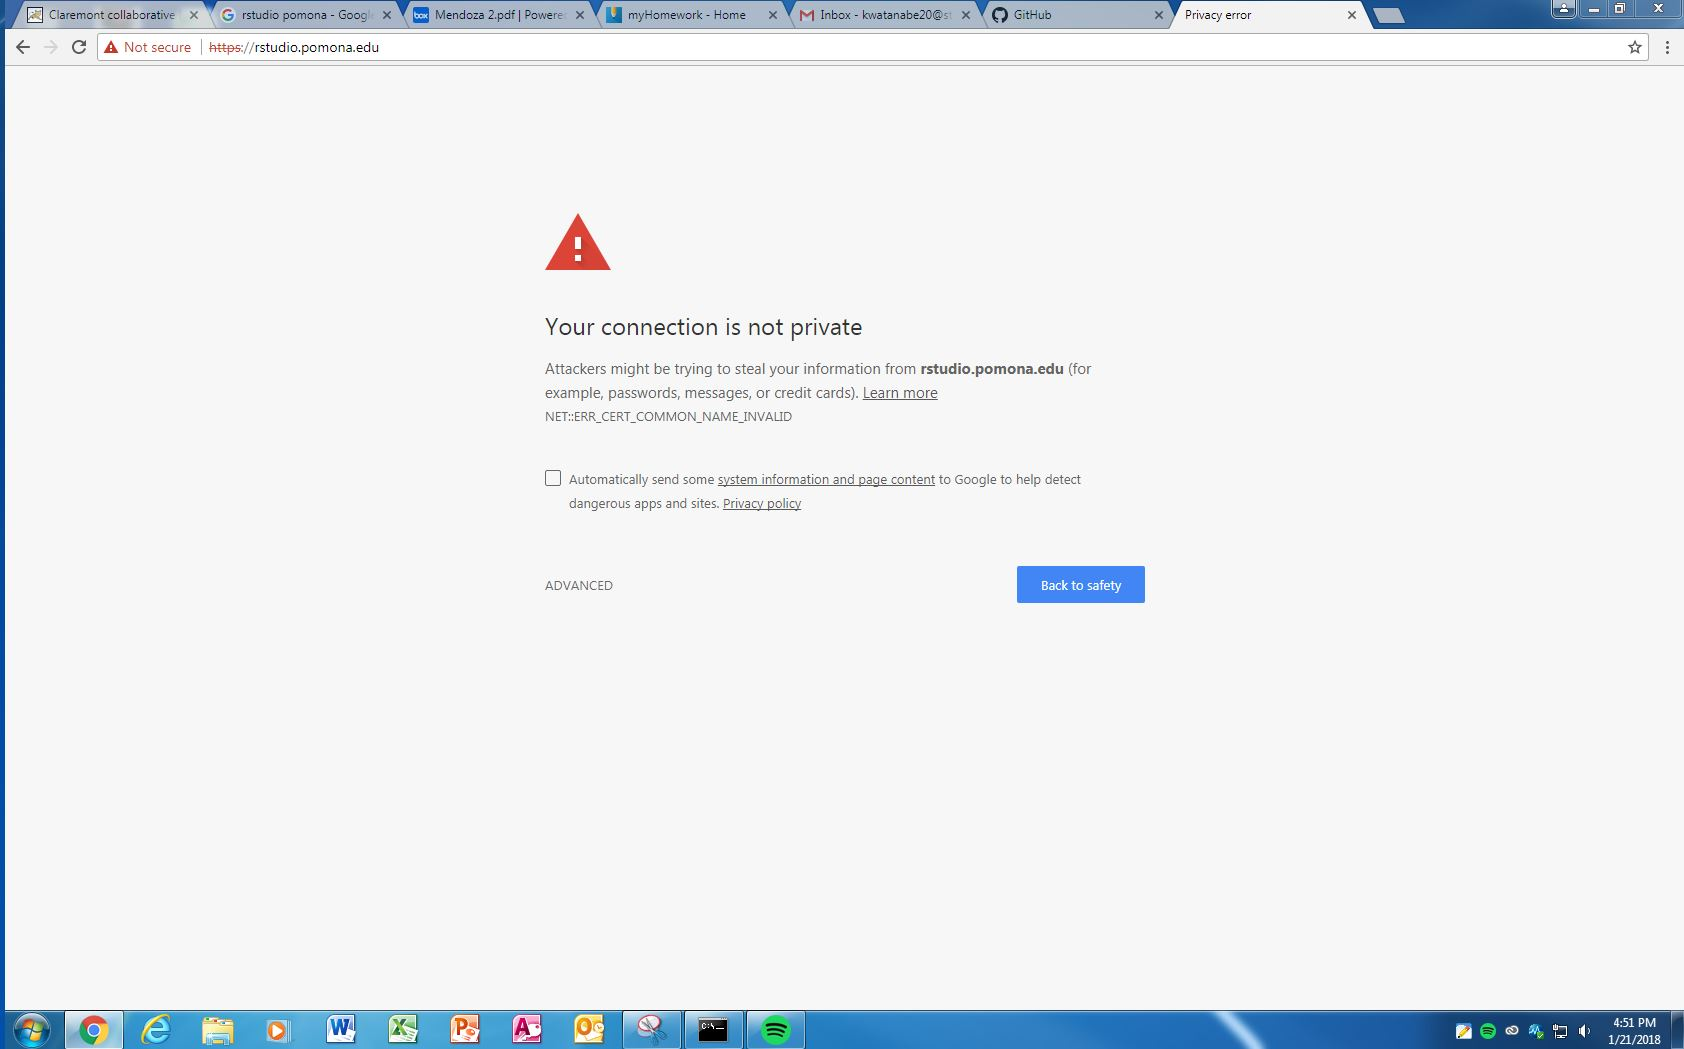
\includegraphics[width=0.99\textwidth]{graphics/Connect_Web_Privacy.JPG}
\caption{Privacy error can be ignored by going to the Advanced settings.}
\label{fig:privacyerror}
\end{figure}


\subsection{4 Rstudio Panels}

Working with Rstudio is a bit confusing at first -- there is lots going on! First, let's unpack the four default pannels that come up when you start Rstudio. 

\NP Each of the panels have tabs, but they can vary depending on what is active in Rstudio. 

\NP To see all of the panels, create the fourth window, we'll need to add create a new text file. Go to File/New File/R Sweave which opens a \LaTeX\ file template. Save the file as "Test.Rnw" and now you have four windows.

\begin{description}
  \item[Upper Left --- Text and Code -- Rnw, \TeX, Txt, and Rmd files] This window usually has the text files you are using to write and edit code and text. If there is not text open, this window will not be present and the console will take up the entire left side. A few things to note: You can have Rnw, Tex, dataframe previews, and text files open in this panel. I suggest you close ones you are not using to avoid working on stuff that you mean to.  
  
  \item[Lower Left -- Console and Compile PDF windows] This is the R console, where you can enter (type directly or submit from the panal above) commands in to R from above. Without a Rmd/Rnw file open this panel might take the entire left side of the program's interface. This is where you can type or submit R commands and were results are displayed. Also, any errors are reported in red here. If you have compiled a LaTeX file, the log file of the process will also be displayed.
  
  \item[Lower Right -- Files/Plots/Packages/Help/Viewer] This panel is handy to see what files are in your workspace, but also shows that packages that have been installed. When you make a plot, it will show up in this panel, but there are times that the plot is too big for the window. You might get a warning if that is the case, where you can usually resize the window to make the plat show up. Finally, it's a handy place to get the help manual to show up. 

  \item[Upper Right -- Environment/History/Git Panel] You can use the ``Environment'' tab to see the files that R as access to. The ``History'' tab displays a history of the commands you have submitted and finally the ''Git'' tab can be used to manage files between the Github server and the local pomona server. 
  
\end{description}

\section{Setting Up Accounts and Communications Keys}

\NP Create Github Account: Go to \href{http:\\github.com}{Github.com} and create an account. I suggest you use your Claremont e-mail adddress because this can come in handy later, should you want to create private repositories, which are free for college students! But you need to make a special request for this (\url{https://education.github.com/discount_requests/new}. For our purposes, you will not need a private repository and you can always request on later. Your email address can be used to prove your student status. 
  

\NP R, Rstudio, and Github can easily be installed on a desktop computer, however, please start by using the server versions via Rstudio. 

\NP Rstudio Server located at \href{http://rstudio.campus.pomona.edu}{\textbf{rstudio.campus.pomona.edu}}. Remember address only works if you are on Pomona's network. 

\NP Login using your Pomona College username and password. This is the address for when you are on campus and using a pomona login name. 

\NP To set up, change Rstudio's weave option to 'knitr'. Navigate to Tools/Global Options/Sweave, then change the 'weave Rnw files' box at the top from Sweave to knitr. This will have minor, but real changes in how files are compiled. Knitr has relatively new and more robust option. Apply and close window. 

\NP If using the downloaded Rstudio, start R Studio from the program files and this will automatically start an R console window.

\subsection{Creating a Connection between Github and RStudio}

\NP Open Rstudio -- which can be either as a local installation or using an RStudio Server via your webbrowser. However for this class, I continue to recommend that you use the RStudio Server.

\NP To use Rstudio's version control, you must create a SSH Key that is used to open a secure connections between RStudio and Github.

\NP To create a Key, follow the Rstudio menus Tools/Global Option and navigate to the `Git/SVN' in the left menu.

\NP ``Create RSA key''. 

\begin{figure}
\centering
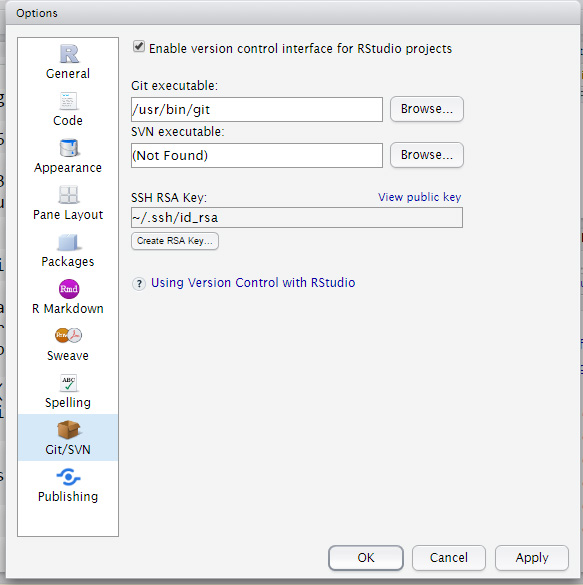
\includegraphics[width=0.6\textwidth]{graphics/CreatingSSH.jpg}
\caption{After natigating through the Rstudio Git/SNV menu, select `Create an RSA Key'.}
\end{figure}

\NP You have the option to create a passphrase. I suggest you ignore this for now, but should you have projects that need extra security, this is a good idea.

\NP After you hit the ``Create'' button an image will be generated in a pop-up window -- As far as I can tell, this image is some sort of encryption thing -- but I don't see any reason why we should care. So, close this pop-up window. 

\NP Next, select the `View the public key' and copy the contents of the pop-up window using ctrl-c. Now we need to paste that key into Github. NOTE: If you closed all the windows, you have to nagivate back to the Git/SVN menu via Global Options. 

\NP Add RSA/SSH Key to Github
  \begin{enumerate}
  \item Go to Profile, in the upper right top of the Github page. Unless you have uploaded a picture of yourself, profile image is a tetris looking icon.
  \item Select the menu item ``Settings.''
  \item Using the left menu, select the ``SSH and GPG keys'' button (Figure~\ref{fig:githubkey}).
  \item Click on new SSH key, type in name of key (e.g. `myRstudio SSH key')
  
\begin{figure}
\centering
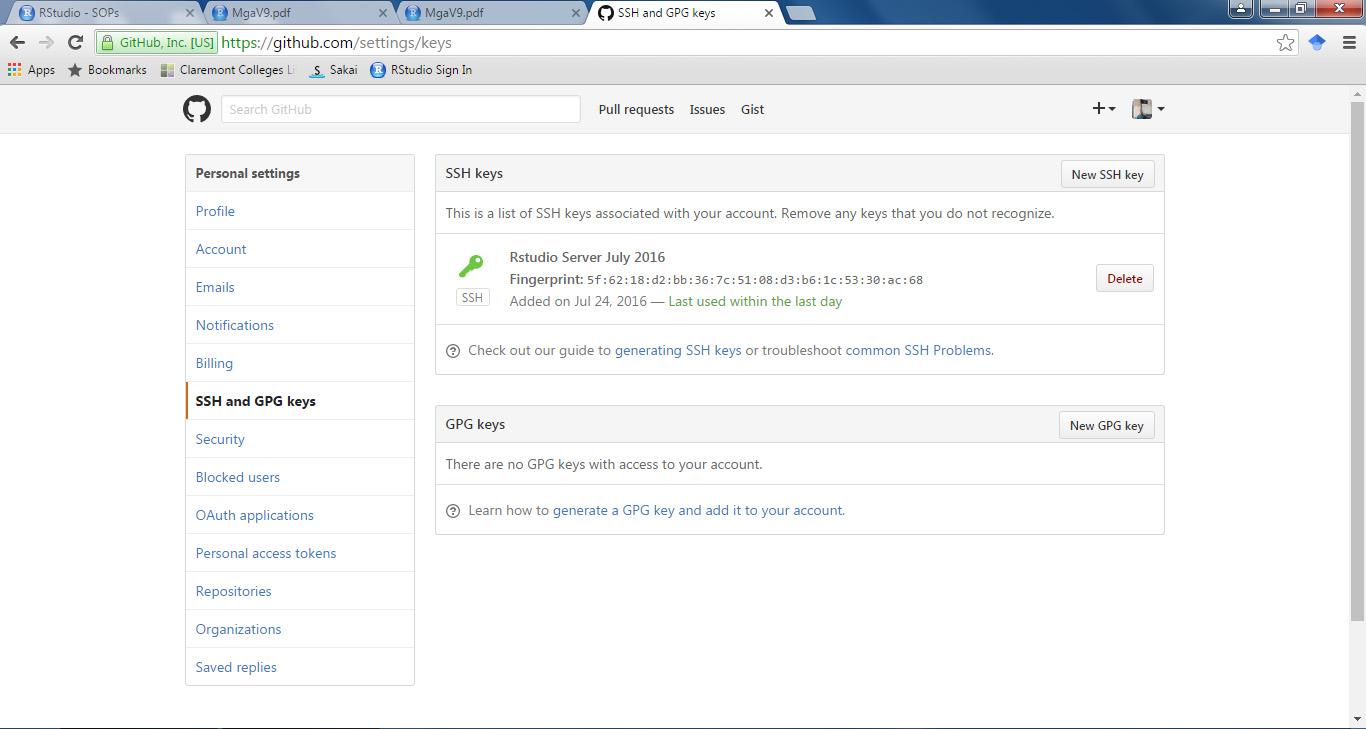
\includegraphics[width=0.7\textwidth]{graphics/Github_SavedSSH.jpg}
\caption{Creating the connection between Rstudio and Gitub requires a `key'. We generate the key in Rstudio and then we tell Github what the key is.}
\label{fig:githubkey}
\end{figure}

  \item Paste in the RSA key, from your clipboard, into the window below.
  \item Hit green ``add SSH key'' button.
  \item Github and R can now communicate.
  \end{enumerate}

\section{Creating and Updating Your Own Repository}

\subsection {How To Create a Fork in Github and Connect It to RStudio}
A fork in GitHub is when you copy someone else’s original repository into your own repository so that when you make edits, you are only making edits in your own pages. When you want to share your changes with the original repository, in this case the marclos/Environmental-Sciences-in-East-Asia repository, you can create a pull request which will be explained in the next set of directions. 

\subsubsection{In Github}
\begin{itemize}
\item To start, you should ne logged into GitHub and have the marclos/Environmental-Sciences-in-East-Asia repository open and you should be logged into RStudio as well. 
\item To create a fork, navigate to the marclos/Environmental-Sciences-in-East-Asia repository home page and look to the top right of the window
  \item Click the button that says “fork” and you should be taken to a new page that has your account name followed by “/Environmental-Sciences-in-East-Asia”
  \item If you see a new page, you have successfully created a new fork where you will make edits from now on 
\end{itemize}

\subsubsection{RStudio}
Now we have to connect your fork to your RStudio account so that all your work can be saved 

\begin{itemize}
  \item Find the green button that says “code” and copy the SSH link 
  \item Then go to RStudio and create a new project
    \item File \rightarrow new project \rightarrow version control \rightarrow Git
  \item Then paste the link you copied into “Repository URL” and give your project a title like “Environmental-Sciences-In-East-Asia-LastName” and save the project in your home directory
    \item You should see a little box pop-up and load a bunch of things onto your RStudio
  \item Scan the bar at the top of your screen until you find the “tools” button, click it and then click shell
  \item In the shell type the following code

    \indent\verb"Git clone" (your SSH link you coped from GitHub earlier)
    
    \indent\verb"Git remote -v"
    
      \item This checks to make sure you correctly cloned the project. You should see something like this: 
        \item Origin git@github.com:erta2020/Environmental-Sciences-in-East-Asia (fetch)
        \item Origin git@github.com:erta2020/Environmental-Sciences-in-East-Asia (push)
    \item Next we need to add Marc’s repository to this project so that you can push and pull later on
      \item Go back to GitHub and under your fork repository name on the top left of your screan, click where it says marclos/Environmental-Sciences-in-East-Asia and you should be taken back to Marc’s page
      \item Click the green code button and copy the SSH link before going back to RStudio
      \item Back in the shell, type the code below
        
        \indent\verb"Git remote add upstream" (the SSH key you just copied)
        
        \indent\verb"Git remote -v"
       
      \item Now you should see four lines, two labeled origin which is your repository and two labeled upstream which is marc’s repository. 
      \item Now you have successfully connected your RStudio to your new GitHub repository 
\end{itemize}

\subsection {How to Create Pull Requests}
You want to make pull requests after you make changes to your work that you want to be reflected in everyone else’s repository. You will need to create a full request to do this. For this class you will make one pull request each week, on Friday’s so that your work can be looked at by Marc over the weekend. 

\subsubsection{Committing The Changes}

\begin{itemize}
\item Click “git” in the top right box and then press commit
  \item After a new window pops up, make sure you click the small square next to the changes you made on the left-hand side 
\item Type a message in the “commit message” box that explains quickly what changes you made, then press commit
  \item Close the pop-up box and press “push” and then once that finishes press “close again” and go back to the main RStudio page
\item Now open GitHub and navigate to your repository 
  \item Click the button that says “pull requests” which will take you to a new page
  \item Click the green “new pull requests” button and you should see the change you just committed in RStudio
  \item Click “create pull request”
  \item Write a similar message that you types in the commit box earlier and finish the request by pressing “create pull request” 
  \item Marc then has the opportunity to review the changes you made and accept them into the main repository so that your classmates can see your new changes
\end{itemize}

\subsection{How to Pull Marc’s Repository Updates Into Your Repository}

This is what you need to do after your classmate’s changes have been added to Marc's main repository. Because you have a fork, the pull requests you make don’t automatically appear to other students in their forks, so you have to pull that information into your fork to make sure that you can also see it. For this class, you will update your RStudio every Monday after Marc has reviewed your Friday pull requests

You can check to see if your Fork is ahead or behind Marc’s repository by going to your GitHub fork and seeing if it says that your branch is ``behind/head marclos by \# of commits''. Once you finish this and if you do everything correctly, your GitHub page will say that your repository Is even with Marc's. 

\subsubsection{Using The Shell in RStudio}
\begin{itemize}
\item In RStudio, open a ``shell'' by looking for the ``tools'' button along the top of your screen and then clicking “shell”
\item Write the following code in the shell, pressing enter before each new bullet point 
  \begin{verbatim}
  \item Git fetch upstream
  \end{verbatim}
    \item This pulls all the updates made in Marc’s repository
  \begin{verbatim}
  \item Git push origin master 
  \end{verbatim}
    \item This finishes the updates and pushes them so they are saved in your repository
\item Press the green “push” button in the top right box under git to make sure everything get’s pushed to GitHub
\end{itemize}

\end{document}
